\section{\texorpdfstring{
\includegraphics[width=150pt]{redux.png}}{Redux}}

\begin{frame}

  \frametitle{Redux}
  Redux is a predictable state container for JavaScript apps.

	\textbf{Three Principles}

	Single source of truth

	State is read-only

	Changes are made with pure functions 

\end{frame}

\begin{frame}

  \frametitle{Architecture of a redux app}
	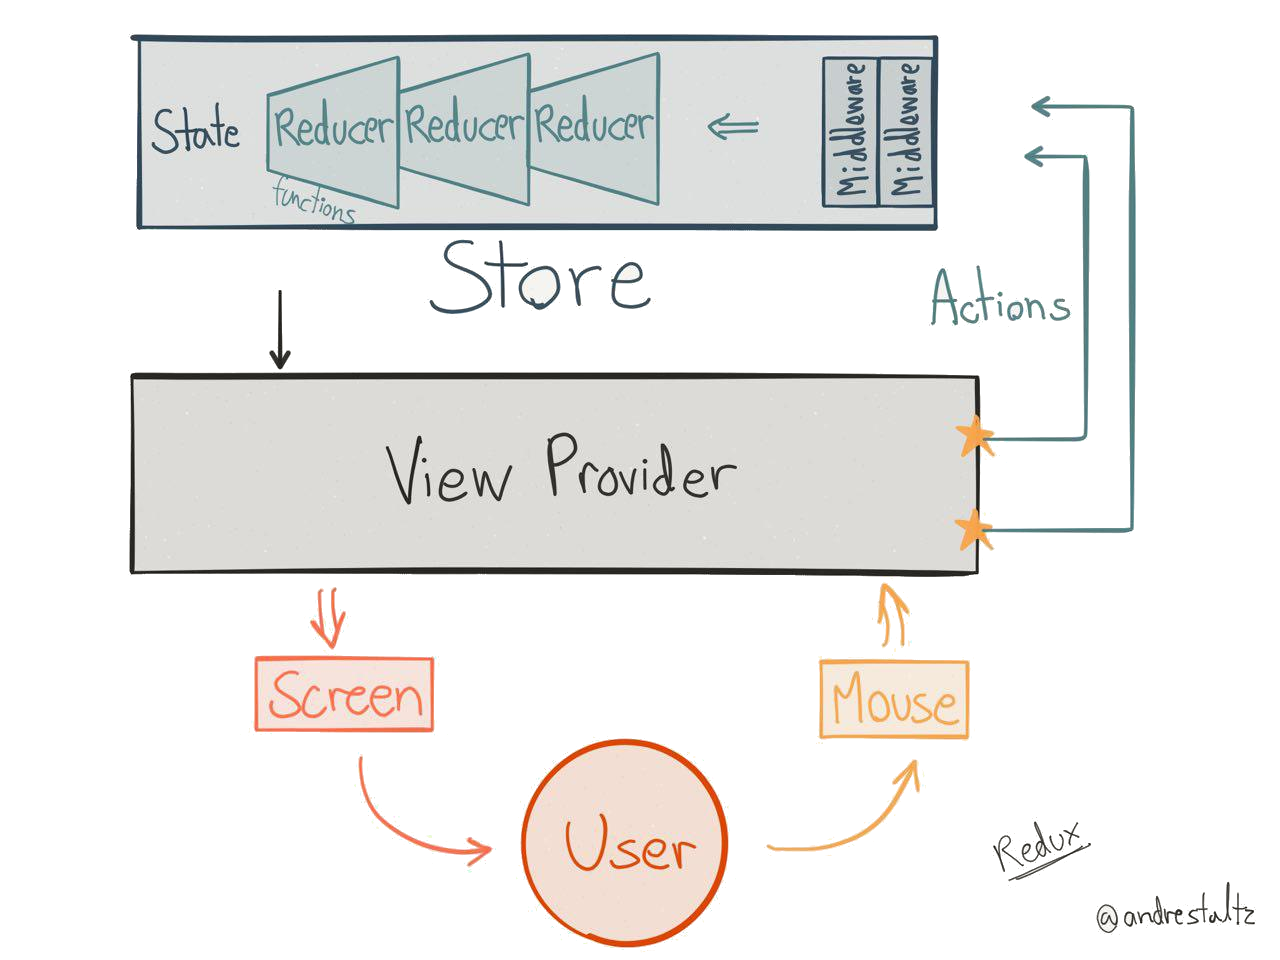
\includegraphics[width=\textwidth]{redux-unidir-ui-arch.png}

\end{frame}

\begin{frame}[fragile]
	\frametitle{Actions}
  Payloads of information that send data from your application to your store. They are the only source of information for the store. You send them to the store using \textit{store.dispatch()}.

	\begin{minted}[fontsize=\tiny]{javascript}
  const action = { type: 'TOGGLE_TODO', index: 6 }  // 'type' is the only thing required
	\end{minted}

  \textbf{Action creators} are functions that return actions

	\begin{minted}[fontsize=\tiny]{javascript}
  function addTodo (text) {
    returns { type: 'ADD_TODO', text }
  }

  store.dispatch(addTodo('Pray to Yisus'))

  const boundAddTodo = text => store.dispatch(addTodo(text))
  boundAddTodo('Pray to Yisus')
	\end{minted}

\end{frame}

\begin{frame}[fragile]
  \frametitle{Reducers}
  Specify how the application's state changes in response to actions.

  \begin{multicols}{2}
  \footnotesize State
	\begin{minted}[fontsize=\tiny]{javascript}
  {
    visibilityFilter: 'SHOW_ALL',
    todos: [
      {
        text: 'Consider using Redux',
        completed: true,
      },
      {
        text: 'Keep all state in a single tree',
        completed: false
      }
    ]
  }
  \end{minted}

  \columnbreak

  \footnotesize Action
	\begin{minted}[fontsize=\tiny]{javascript}
  {
    type: 'SET_VISIBILITY_FILTER',
    filter: 'SHOW_FINISHED'
  }
  \end{minted}

  \end{multicols}
\end{frame}

\begin{frame}[fragile]
  \frametitle{Reducers}

\small The reducer is a pure function \textit{(previousState, action) => newState}

\begin{minted}[fontsize=\tiny]{javascript}
function todoApp (state = initialState, action) {  // initializes the state
  switch (action.type) {  // looks the type of the action
    case SET_VISIBILITY_FILTER:
      return Object.assign({}, state, {  // returns the new state object
        visibilityFilter: action.filter  // with the changed visibility filter
      })
    case ADD_TODO:
      return Object.assign({}, state, {
        todos: [
          ...state.todos,
          {
            text: action.text,
            completed: false
          }
        ]
      })    
    default:
      return state
  }
}
\end{minted}

\end{frame}



\begin{frame}[fragile]
\frametitle{Reducers composition}

\begin{multicols}{2}
\scriptsize One reducer for each part of the tree
\begin{minted}[fontsize=\tiny]{javascript}
function todos (state = [], action) {
  switch (action.type) {
    case ADD_TODO:
      return [
        ...state,
        {
          text: action.text,
          completed: false
        }
      ]
    default:
      return state
  }
}

function visibilityFilter(
    state = SHOW_ALL, action
  ) {
  switch (action.type) {
    case SET_VISIBILITY_FILTER:
      return action.filter
    default:
      return state
  }
}
\end{minted}

\columnbreak

\scriptsize All the reducers are combined in one
\begin{minted}[fontsize=\tiny]{javascript}
function todoApp (state = {}, action) {
  return {
    visibilityFilter: visibilityFilter(
      state.visibilityFilter, action),
    todos: todos(state.todos, action)
  }
}

// Redux let's us do it with combineReducers

import { combineReducers } from 'redux'

const todoApp = combineReducers({
  visibilityFilter,
  todos
})

\end{minted}

\end{multicols}
\end{frame}
